\chapter{Wdrożenie i prezentacja działania}
\thispagestyle{chapterBeginStyle}

W tym rozdziale została przedstawiona instrukcja obsługi niniejszej platformy. W pierwszej części omówiono wymagania, które muszą zostać spełnione, aby framework z przykładowymi danymi był gotów do pracy, następnie opisano czynności instalacyjne. 
W dalszej części rozdziału umieszczono prezentację działania wybranych funkcjonalności, podzieloną ze względu na zdefiniowanych aktorów. 

%W tym rozdziale należy omówić zawartość pakietu instalacyjnego oraz założenia co do środowiska, w którym realizowany system będzie instalowany. Należy przedstawić procedurę instalacji i wdrożenia systemu. Czynności instalacyjne powinny być szczegółowo rozpisane na kroki. Procedura wdrożenia powinna obejmować konfigurację platformy sprzętowej, OS (np. konfiguracje niezbędnych sterowników) oraz konfigurację wdrażanego systemu, m.in.\ tworzenia niezbędnych kont użytkowników. Procedura instalacji powinna prowadzić od stanu, w którym nie są zainstalowane żadne składniki systemu, do stanu w którym system jest gotowy do pracy i oczekuje na akcje typowego użytkownika.%
\section{Wymagania początkowe}

\section{Instalacja aplikacji}

\section{Prezentacja wybranych funkcjonalności}

W ramach tej sekcji zostaną przedstawione najważniejsze funkcjonalności systemu, które pojawiły się w rozdziale \textbf{Projekt systemu}.  

\subsection{Funkcjonalności przewidziane dla administratora sklepu}
Sekcja ta ma za zadanie pokazać w praktyce deklarowaną wcześniej elastyczność systemu, czyli to,jak programista może skonfigurować platformę pod potrzeby sklepu, który implementuje.

\subsubsection{Widok panelu administracyjnego}
Na rysunku \ref{scr_adminmain} został przedstawiony panel administracyjny. Literkami A, B, C i D oznaczono ważne elementy. \textbf{A} -- konfigurowalne menu, \textbf{B} -- dynamiczna tabela encyjna ze wszystkim encjami rodzaju \texttt{price} (tabela cen). \textbf{C} przycisk dodania nowego egzemplarza encji, \textbf{D} -- linki z ID przekierowują do dynamicznego formularza edycji encji. 
\begin{figure}
	\begin{center}
		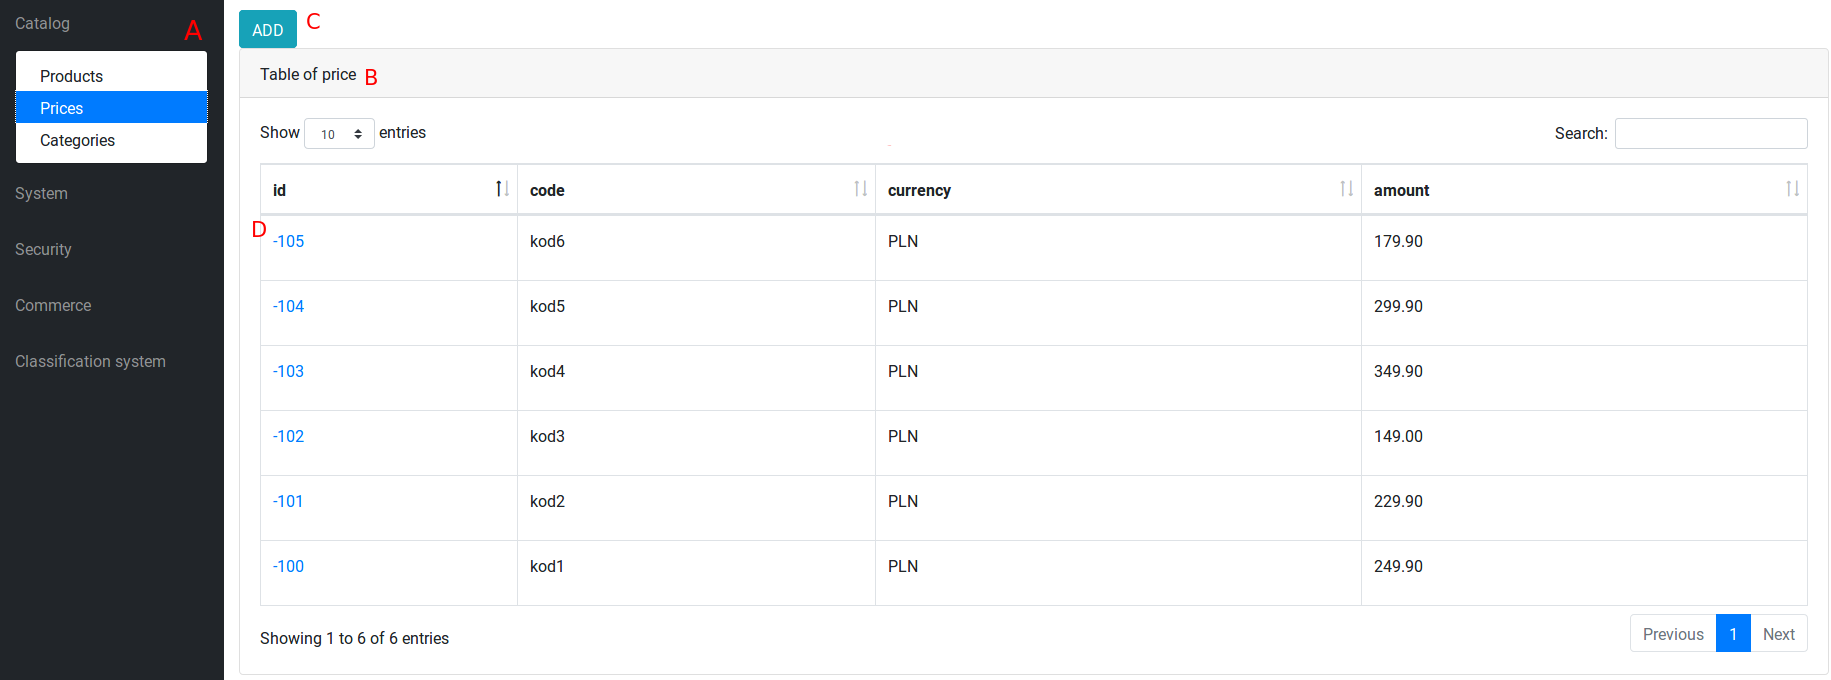
\includegraphics[width=1\textwidth]{admin-main.png}
	\end{center}
	\caption{{\color{black}Widok panelu administracyjnego}} \label{scr_adminmain}
\end{figure}

\subsubsection{Zmiana właściwości encji} 
Zmiana właściwości dowolnej encji zostanie przedstawiona na podstawie produktu.
 
\noindent
\textbf{Scenariusz: } zmiana ceny. \textbf{Rysunek: } \ref{zmianacenyproduktu} 
\begin{itemize}
	\item wybierz z tabeli encyjnej dowolny produkt i wejdź w szczegóły (1)
	\item w dynamicznym formularzu spośród relacji produktu wybierz cenę (price) i wejdź w szczegóły (2) 
	\item w formularzu edycji ceny zmień jej wartość i naciśnij \textit{submit}(3)
	\item po powrocie do edycji produktu zostanie wyświetlona zmieniona cena (4)
\end{itemize}
\begin{figure}
	\begin{center}
		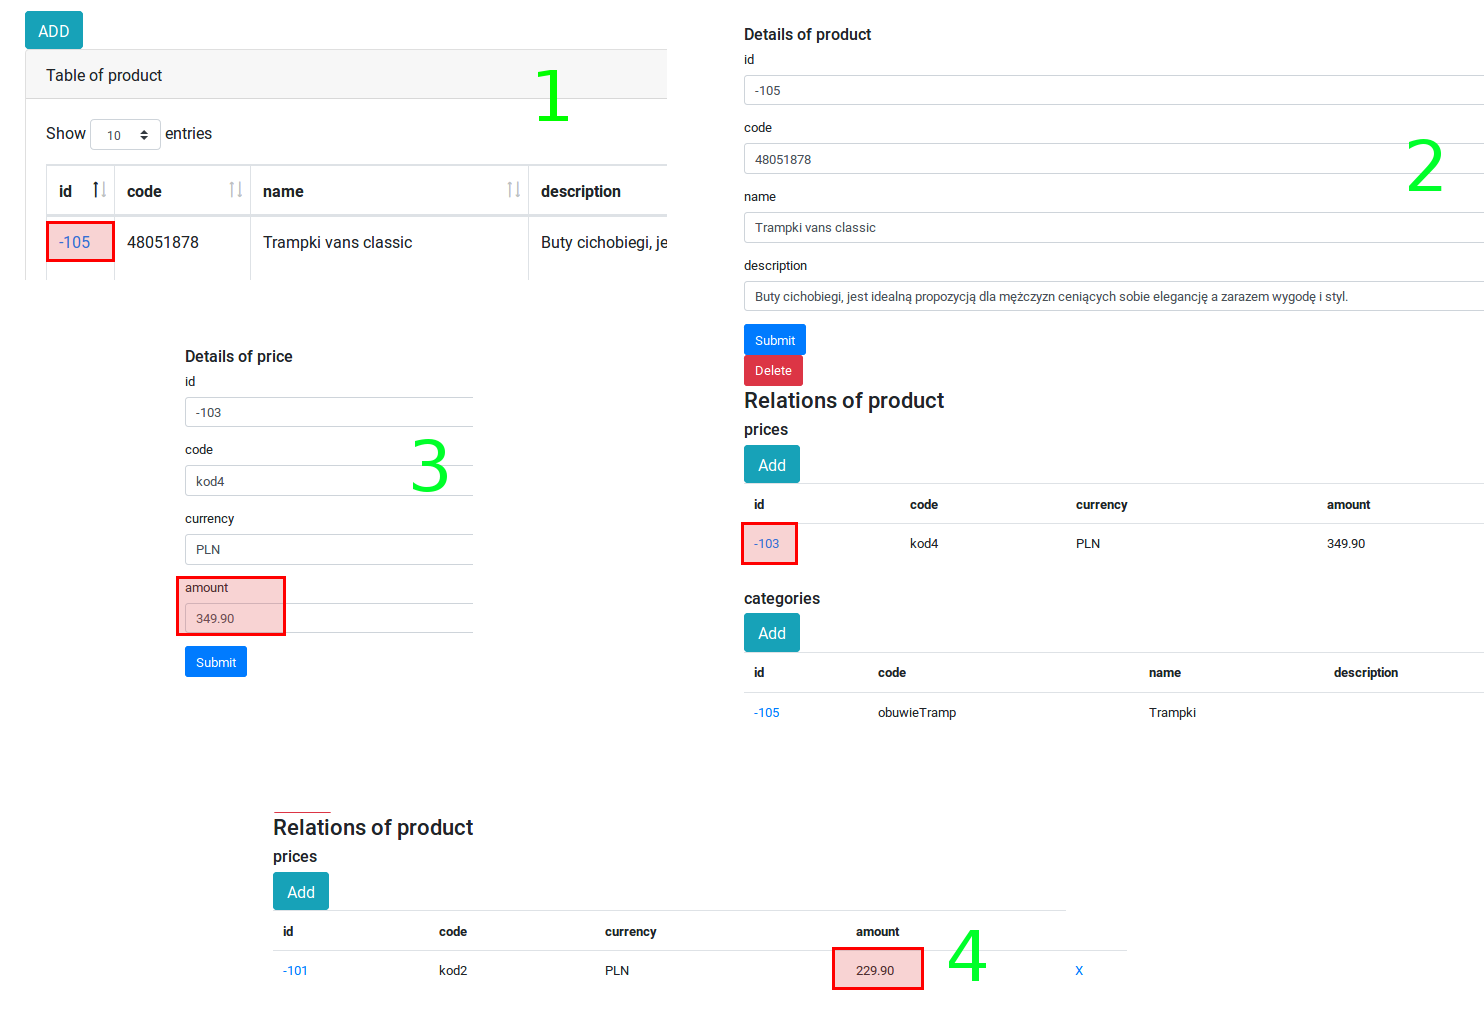
\includegraphics[scale=1.3]{zmianacenyproduktu.png}
	\end{center}
	\caption{{\color{black}Zmiana ceny w produkcie}} \label{zmianacenyproduktu}
\end{figure}


\subsection{Funkcjonalności przewidziane dla programisty}
Sekcja ta ma za zadanie pokazać w praktyce deklarowaną wcześniej elastyczność systemu, czyli to,jak programista może skonfigurować platformę pod potrzeby sklepu, który implementuje. 
\subsubsection{Dodanie encji do systemu}









